\newpage
\subsection{Cálculo das Posições: Cinemática Direta e Inversa}

Para o desenvolvimento da modelagem cinemática do manipulador serial de 6 GDL, foi utilizada a convenção de Denavit-Hartenberg (DH), amplamente empregada na representação matemática de robôs manipuladores. O modelo adotado foi baseado no manipulador industrial \textit{Stäubli TX90}, conforme apresentado no TCC utilizado como referência.

\subsubsection{Parâmetros de Denavit-Hartenberg}

A partir das dimensões geométricas e dos sistemas de coordenadas definidos na Figura \ref{diagrama_staubli}, é possível determinar os parâmetros de Denavit-Hartenberg que descrevem a relação espacial entre os elos e juntas do manipulador. A convenção DH permite representar a cinemática do robô por meio dos parâmetros $a_i$, $\alpha_i$, $d_i$ e $\theta_i$, os quais são obtidos diretamente da geometria apresentada abaixo. 
A seguir, estão representadas as dimensões do braço robótico e a convenção adotada para cada junta, respectivamente.

\begin{figure}[H]
    \centering
    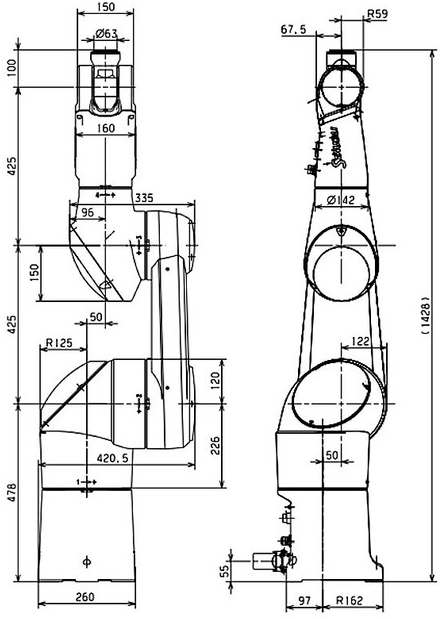
\includegraphics[width=0.5\linewidth]{Imagens/dimensoes_tx90.png}
    \caption{Dimensões do braço Stäubli TX90}
    \label{dimensoes_staubli}
\end{figure}

\begin{figure}[H]
    \centering
    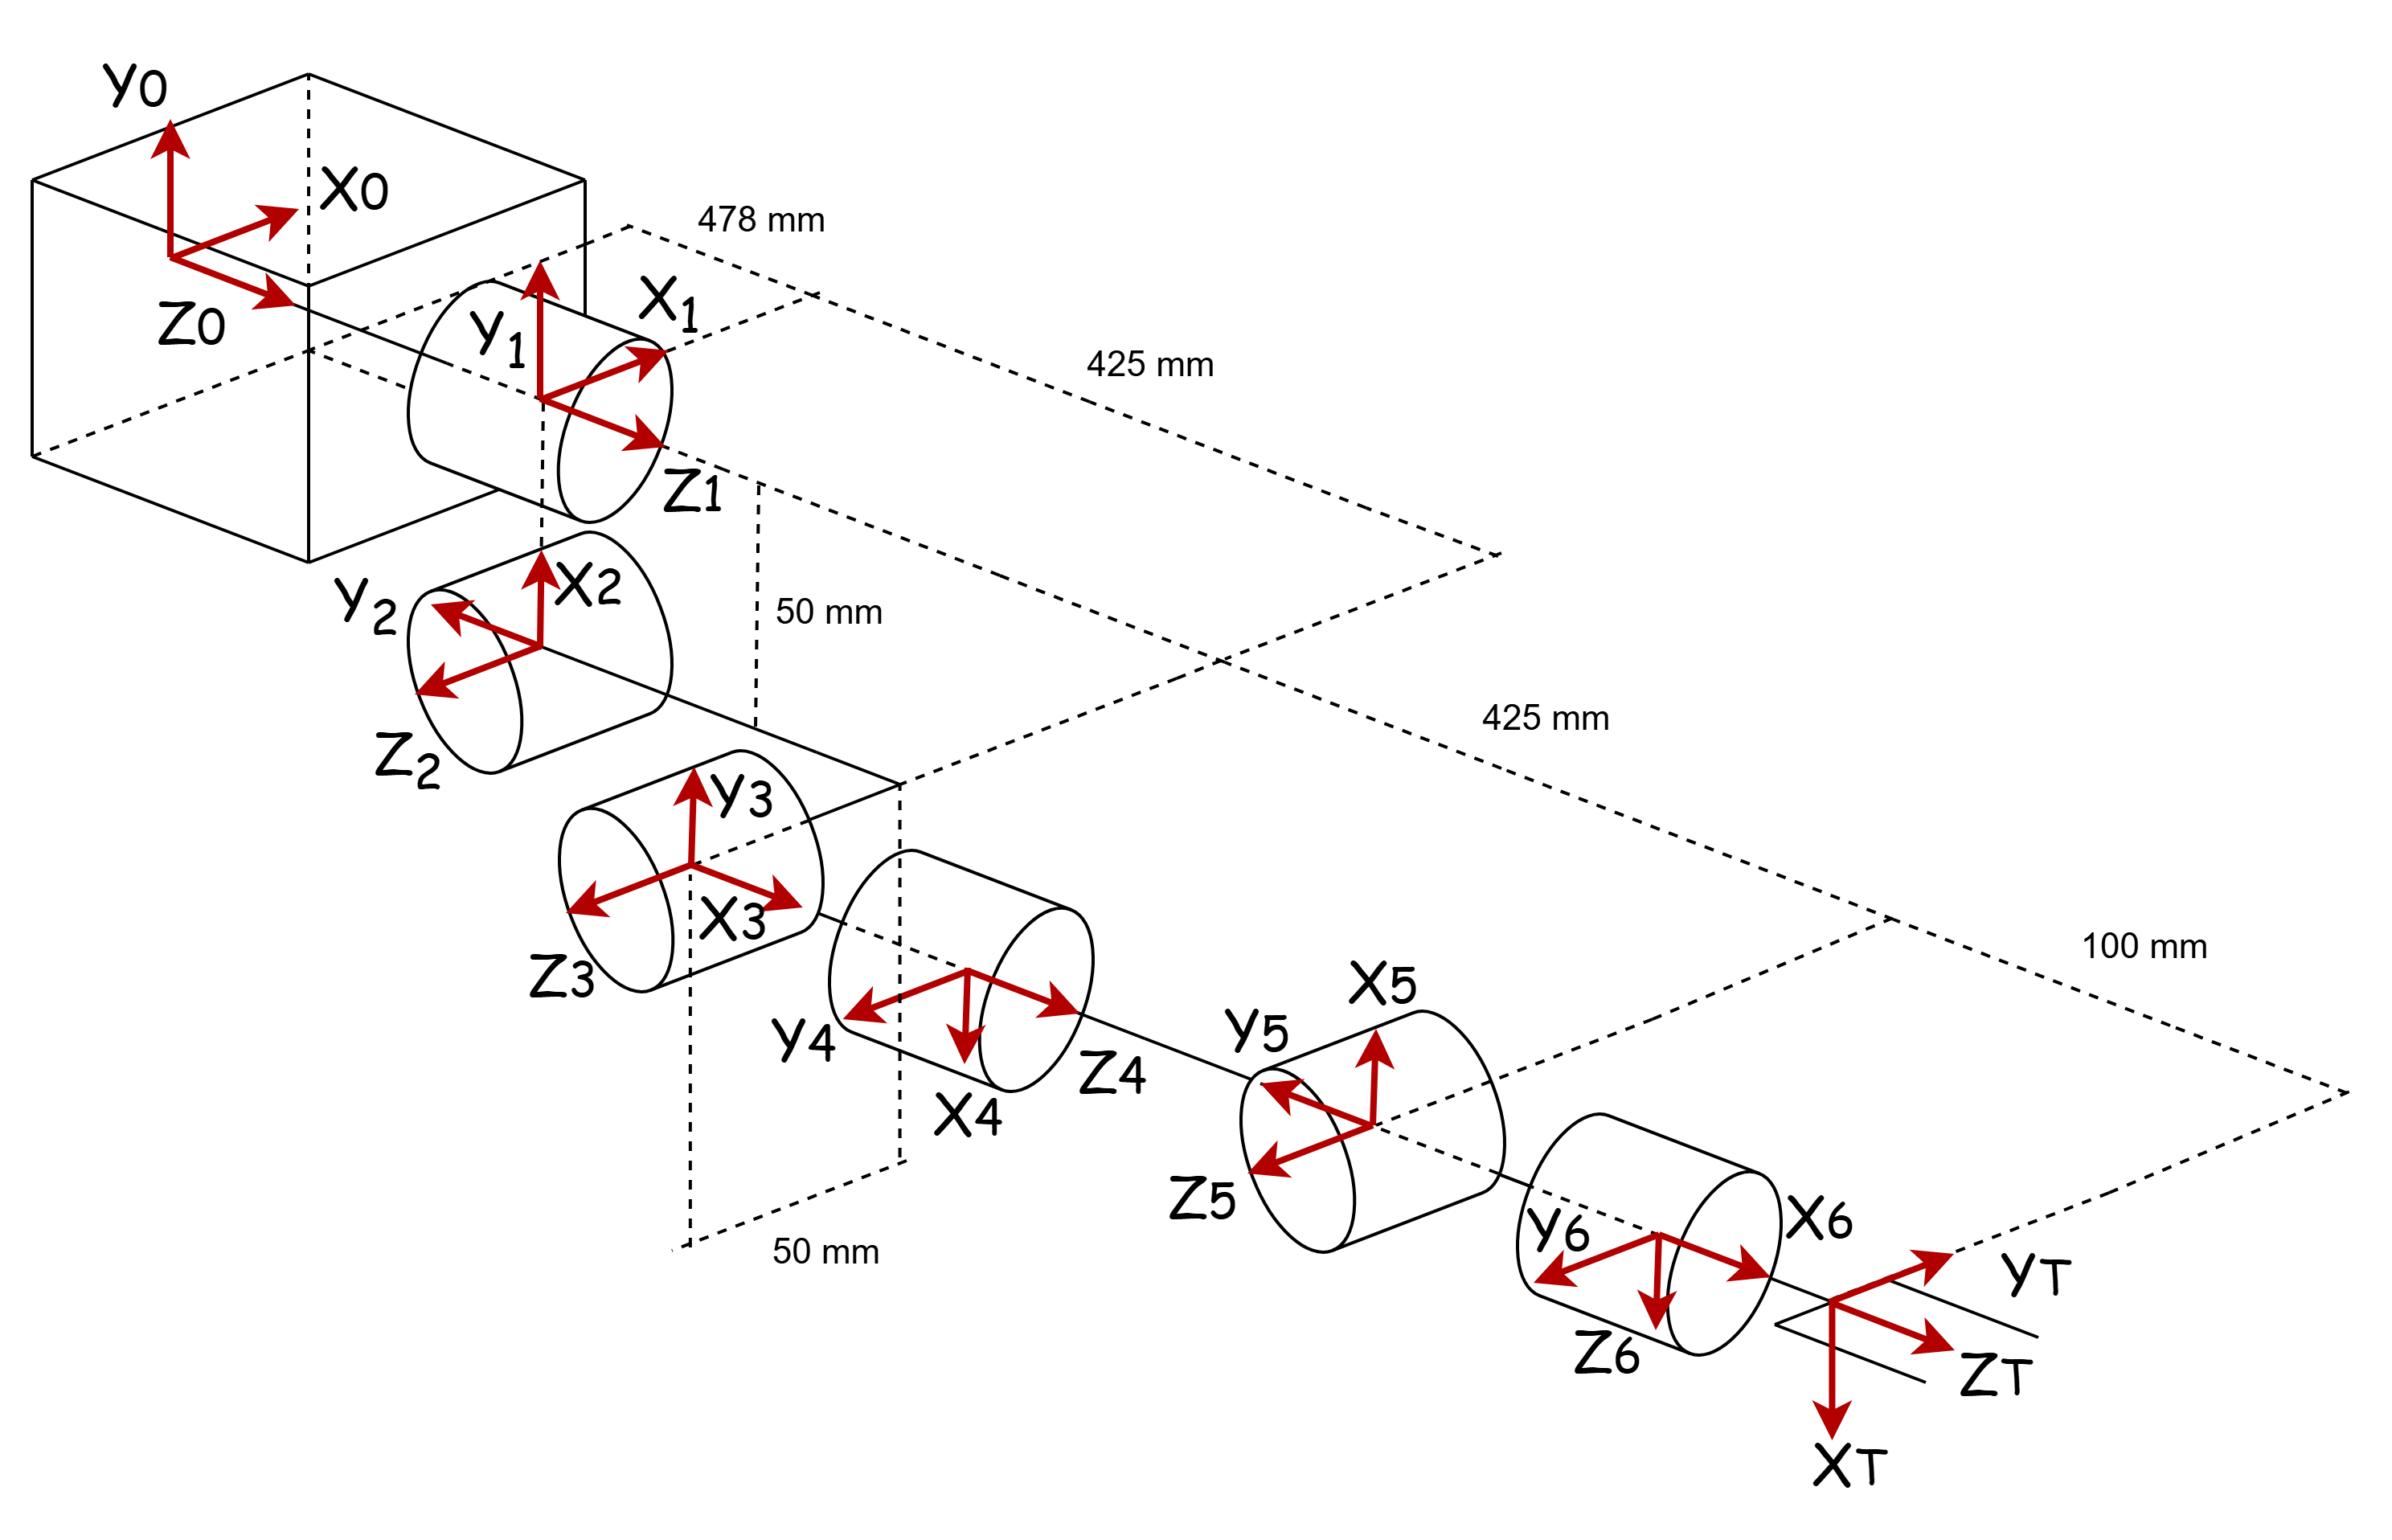
\includegraphics[width=0.75\linewidth]{Imagens/diagrama_staubli_2.png}
    \caption{Modelo esquemático do Stäubli TX90}
    \label{diagrama_staubli}
\end{figure}

\par No diagrama acima, vale ressaltar que as distâncias entre as juntas 3 e 4 e as juntas 5 e 6 são nulas. A Tabela \ref{tab:dh} apresenta os parâmetros DH utilizados para descrever geometricamente o manipulador. 

\begin{table}[H]
\centering
\caption{Parâmetros de Denavit-Hartenberg}
\label{tab:dh}
\begin{tabular}{ccccc}
\hline
Junta & $a_i$ (mm) & $\alpha_i$ (rad) & $d_i$ (mm) & $\theta_i$ \\
\hline
1 & 0  & 0 & 478 & $\theta_1$ \\
2 & -50 & $-\frac{\pi}{2}$ & 0 & $\theta_2 + \frac{\pi}{2}$ \\
3 & 425 & 0  & 50   & $\theta_3 - \frac{\pi}{2}$\\
4 & 0   & $-\frac{\pi}{2}$ & 0   & $\theta_4 - \frac{\pi}{2}$ \\
5 & 0   & $-\frac{\pi}{2}$  & 425   & $\theta_5 + \frac{\pi}{2}$ \\
6 & 0   & $-\frac{\pi}{2}$ & 0 & $\theta_6 + \frac{\pi}{2}$ \\
\hline
\end{tabular}
\end{table}

Para este caso, há também uma medida de 100 mm que vai da junta 6 até garra. Como a garra não é uma junta, ela não pôde ser adicionada diretamente na tabela DH. No entanto, para realizar essa compensação da distância da junta até a garra, podemos adicionar uma transformação independente ao robô, como a seguir.

\begin{equation}
H_6^{Tool} =
\begin{bmatrix}
1 & 0 & 0 & 0 \\
0 & 1 & 0 & 0 \\
0 & 0 & 1 & 100 \\
0 & 0 & 0 & 1
\end{bmatrix}
\end{equation}

\subsubsection{Cinemática Direta}

A cinemática direta tem como objetivo determinar a posição e orientação do efetuador final a partir dos ângulos das juntas do manipulador. A matriz homogênea de transformação entre dois referenciais consecutivos é dada por:

\begin{equation}
H_{i-1}^i =
R_{z,\theta_i}
\cdot
T_{z,d_i}
\cdot
T_{x,a_i}
\cdot
R_{x,\alpha_i}
\end{equation}

Resultando na forma geral:

\begin{equation}
H_i^ {i-1} =
\begin{bmatrix}
\cos\theta_i &
-\sin\theta_i \cos\alpha_i &
\sin\theta_i \sin\alpha_i &
a_i \cos\theta_i \\
\\
\sin\theta_i &
\cos\theta_i \cos\alpha_i &
-\cos\theta_i \sin\alpha_i &
a_i \sin\theta_i \\
\\
0 &
\sin\alpha_i &
\cos\alpha_i &
d_i \\
\\
0 & 0 & 0 & 1
\end{bmatrix}
\end{equation}

A matriz homogênea total do manipulador é obtida pela multiplicação das matrizes individuais, incluindo a referente a ferramenta:

\begin{equation}
H_0^{Tool} =
H_0^1
\cdot
H_1^2
\cdot
H_2^3
\cdot
H_3^4
\cdot
H_4^5
\cdot
H_5^6
\cdot
H_6^{Tool}
\end{equation}

A matriz homogênea final possui a seguinte estrutura:

\begin{equation}
H_0^{Tool} =
\begin{bmatrix}
R(q) & P(q) \\
0 & 1
\end{bmatrix}
\end{equation}

Onde:

\begin{equation}
P(q)=
\begin{bmatrix}
P_x \\
P_y \\
P_z
\end{bmatrix}
\end{equation}

representa a posição do efetuador final, enquanto:

\begin{equation}
R(q)=
\begin{bmatrix}
l_x & m_x & n_x \\
l_y & m_y & n_y \\
l_z & m_z & n_z
\end{bmatrix}
\end{equation}

representa a orientação do efetuador.

Para a validação do modelo, considerou-se a seguinte configuração angular:

\begin{equation}
q =
\begin{bmatrix}
0^\circ \\
0^\circ \\
0^\circ \\
0^\circ \\
0^\circ \\
0^\circ
\end{bmatrix}
\end{equation}

Com isso, foram obtidos as seguintes matrizes de transformação homogêneas.

\begin{equation}
H_0^1=
\begin{bmatrix}
1 & 0 & 0 & 0\\
0 & 1 & 0 & 0\\
0 & 0 & 1 & 478\\
0 & 0 & 0 & 1
\end{bmatrix}
\end{equation}

\begin{equation}
H_1^2=
\begin{bmatrix}
0 & 0 & 1 & 0\\
1 & 0 & 0 & -50\\
0 & -1 & 0 & 0\\
0 & 0 & 0 & 1
\end{bmatrix}
\end{equation}

\begin{equation}
H_2^3=
\begin{bmatrix}
0 & 1 & 0 & 0\\
-1 & 0 & 0 & -425\\
0 & 0 & 1 & 50\\
0 & 0 & 0 & 1
\end{bmatrix}
\end{equation}

\begin{equation}
H_3^4=
\begin{bmatrix}
0 & 0 & 1 & 0\\
-1 & 0 & 0 & 0\\
0 & -1 & 0 & 0\\
0 & 0 & 0 & 1
\end{bmatrix}
\end{equation}

\begin{equation}
H_4^5=
\begin{bmatrix}
1 & 0 & 0 & 0\\
0 & 0 & 1 & 0\\
0 & -1 & 0 & 425\\
0 & 0 & 0 & 1
\end{bmatrix}
\end{equation}

\begin{equation}
H_5^6=
\begin{bmatrix}
1 & 0 & 0 & 0\\
0 & 0 & 1 & 0\\
0 & -1 & 0 & 0\\
0 & 0 & 0 & 1
\end{bmatrix}
\end{equation}

\begin{equation}
H_6^{Tool}=
\begin{bmatrix}
1 & 0 & 0 & 0\\
0 & 1 & 0 & 0\\
0 & 0 & 1 & 100\\
0 & 0 & 0 & 1
\end{bmatrix}
\end{equation}

Substituindo os valores nas matrizes de transformação, obteve-se a posição do efetuador:

\begin{equation}
P(q)=
\begin{bmatrix}
-50 \\
-50 \\
1428
\end{bmatrix}
\text{ mm}
\end{equation}

e a orientação:

\begin{equation}
R(q)=
\begin{bmatrix}
0 & 1 & 0 \\
-1 & 0 & 0 \\
0 & 0 & 1
\end{bmatrix}
\end{equation}

Para visualização do resultado, foi desenvolvido um código em matlab, com o objetivo de visualizar a posição do efetuador no espaço.
\begin{figure}[H]
    \centering
    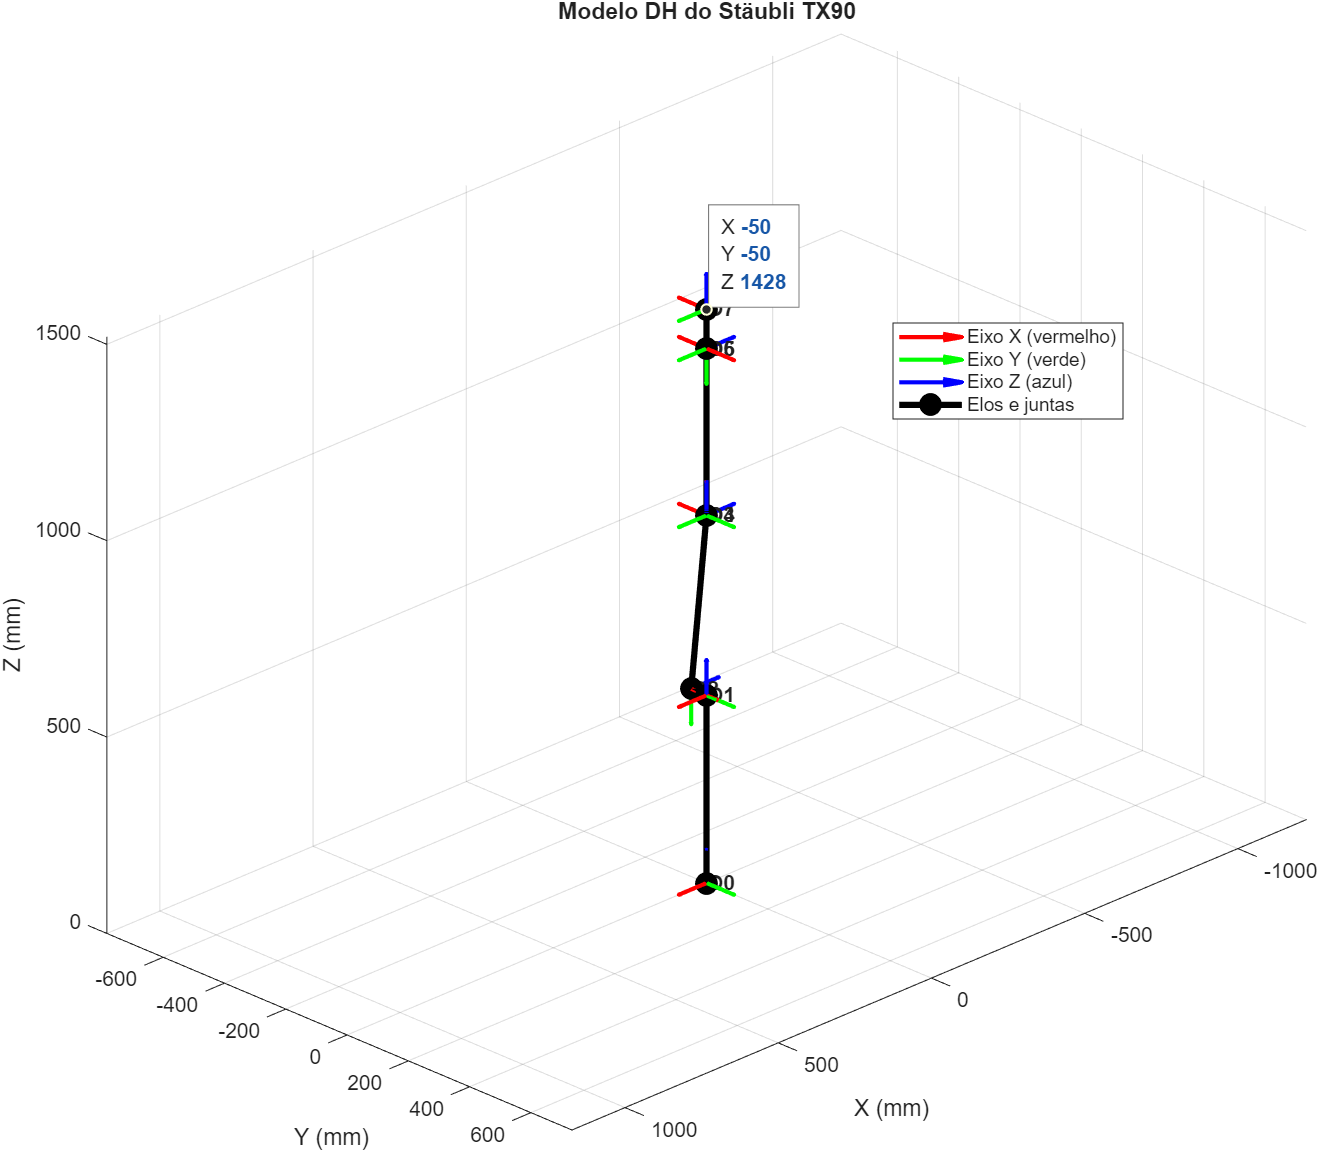
\includegraphics[width=0.5\linewidth]{Imagens/modelo_staubli_matlab.png}
    \caption{Modelo do TX90 visto no MATLAB}
\end{figure}

\subsubsection{Cinemática Inversa}

A cinemática inversa consiste em determinar os ângulos das juntas necessários para atingir uma determinada posição e orientação do efetuador final.

Foi utilizado o método de desacoplamento cinemático, separando o problema em:

\begin{itemize}
    \item Cinemática inversa de posição;
    \item Cinemática inversa de orientação.
\end{itemize}

\begin{figure}[H]
    \centering
    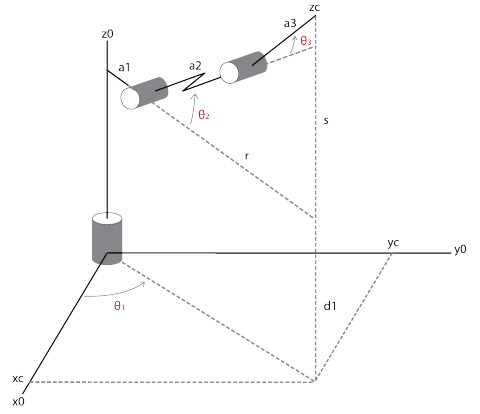
\includegraphics[width=0.5\linewidth]{Imagens/modelo-cinematica_inversa.png}
    \caption{Modelo para cinemática inversa}
\end{figure}

Inicialmente, calcula-se o centro do pulso do manipulador:

\begin{equation}
P_c =
P - d_6 R
\begin{bmatrix}
0 \\
0 \\
1
\end{bmatrix}
\end{equation}

A partir disso, determina-se o primeiro ângulo:

\begin{equation}
\theta_1 = atan2(P_{cy}, P_{cx})
\end{equation}

Para obtenção de $\theta_3$, aplica-se a Lei dos Cossenos:

\begin{equation}
D =
\frac{
P_{cx}^2 + P_{cy}^2 + (P_{cz}-d_1)^2
- a_2^2 - a_3^2
}{
2a_2a_3
}
\end{equation}

\begin{equation}
\theta_3 =
atan2(\pm \sqrt{1-D^2}, D)
\end{equation}

O ângulo $\theta_2$ é calculado por:

\begin{equation}
\theta_2 =
atan2(P_{cz}-d_1,\sqrt{P_{cx}^2+P_{cy}^2})
-
atan2(a_3\sin\theta_3,
a_2+a_3\cos\theta_3)
\end{equation}

Após determinar os três primeiros ângulos, calcula-se a matriz de orientação do pulso:

\begin{equation}
R_3^6 =
(R_0^3)^{-1}R
\end{equation}

Por fim, os ângulos do pulso são obtidos através das relações trigonométricas:

\begin{equation}
\theta_5 = atan2(\sqrt{1-i^2}, i)
\end{equation}

\begin{equation}
\theta_6 =
atan2
\left(
\frac{h}{\sin\theta_5},
\sqrt{1-\left(\frac{h}{\sin\theta_5}\right)^2}
\right)
\end{equation}

\begin{equation}
\theta_4 =
atan2
\left(
\frac{f}{\sin\theta_5},
\sqrt{1-\left(\frac{f}{\sin\theta_5}\right)^2}
\right)
\end{equation}

Os resultados obtidos pela cinemática inversa coincidiram com os valores originalmente utilizados na cinemática direta, validando matematicamente o modelo desenvolvido.